\section{Experimentaci\'on} \label{section:Experimentation}

Con el objetivo de comprobar la viabilidad y funcionamiento del prototipo implementado se propone la evaluaci\'on 
de su comportamiento ante dos escenarios de prueba. Los experimentos se dividen en fases. La primera fase verifica 
la correctitud del proceso de exploraci\'on efectuado por el Crawler y creaci\'on de la base de datos de Neo4j en el  
Cat\'alogo de Datos para la fuente de datos de turno. La segunda fase consiste en la creaci\'on 
del grafo de join y \'arboles de join. La tercera fase consiste en la generaci\'on de las consultas dado una 
definici\'on de esquema 
estrella mediante un script del DSL y la selecci\'on de los joins efectuada por el usuario. La cuarta fase y \'ultima 
es la validaci\'on de las consultas generadas 
mediante la creaci\'on manual de un pipeline de poblaci\'on a partir de las mismas y su ejecución. Todos los archivos que intervienen 
en el proceso de experimentaci\'on se encuentran en la carpeta \textbf{experiments} en el directorio ra\'iz del proyecto. 
Cada experimento posee su propia carpeta en las cuales existen tres scripts de python y un scripts del DSL que constituye 
la definición del esquema estrella a poblar. Los scripts de python tienen el mismo nombre en ambas carpetas de experimentaci\'on, 
\textbf{create.py}, \textbf{populate.py}, \textbf{pipeline.py}. El primero se encarga de 
crear la base de datos correspondiente al escenario de ventas minoristas descrito anteriormente. El segundo se 
encarga de poblar dicha base de datos. El tercero es la implementaci\'on de un pipeline de poblaci\'on utilizando 
las consultas generadas. Los scripts utilizan las librerias de python SQLAlchemy, Psycopg2 y Faker para llevar a 
cabo sus tareas. En particular, la biblioteca de python Faker proporciona facilidades para la generaci\'on de informaci\'on, 
la cual es utilizada para poblar las bases de datos de prueba. A continuaci\'on se describen 
los detalles de los experimentos.

\subsection{Ambiente de experimentaci\'on}

\subsubsection{Equipo}

Se utilizó una computadora portátil con un procesador Intel(R) Core(TM) i7-11370H 11th Gen @ 3.30GHz, 16GB de 
memoria RAM y sistema operativo Windows 11 Home 23H2.

\subsubsection{Docker}

Se utilizó Docker para simular el traspaso de datos por red entre la aplicaci\'on, el Cat\'alogo de Datos y 
los servidores de bases de datos fuente y destino. Se crea una imagen de la aplicaci\'on basada en python:3.10, con el 
nombre \textbf{autoetl}. 
Con el archivo \textbf{docker-compose.yml} se inicializan todos los contenedores que intervienen en el proceso 
de experimentaci\'on. Los servidores de bases de datos fuente y destino son contenedores de PostgreSQL llamados 
\textbf{db} y \textbf{target} respectivamente. El Cat\'alogo de Datos es un contenedor de Neo4j con nombre 
\textbf{data\_catalog}. La aplicaci\'on implementada yace en un contenedor de la imagen creada \textbf{autoetl}. 
Por \'ultimo, con el objetivo de visualizar los resultados del proceso de poblaci\'on se añade al ambiente un 
contenedor de \textbf{pgadmin4}, el cual proporciona una herramienta para la visualizaci\'on de bases de datos 
de PostgreSQL.

\subsection{Experimento 1: Escenario de ventas minoristas}

Este escenario se basa en \textbf{Retail Sales} expuesto en el Cap\'itulo 2
de \cite{kimball2011data}. 

Una red de tiendas cuenta con sucursales distribuidas en varias provincias del país. Estas tiendas se encuentran ubicadas 
en diferentes barrios de los municipios de cada provincia. Las tiendas se dividen en departamentos y cada uno vende 
una serie de productos. Se almacenan los detalles de las transacciones realizadas, es decir, las ventas. Para cada venta, se guarda 
el producto vendido, la tienda en la que se realizó, la fecha de la transacción, la cantidad vendida y el monto pagado.
La figura \ref{fig:retail-transactional} muestra las tablas del sistema transaccional y la relación entre ellas.

\begin{figure}[ht]
    \centering
    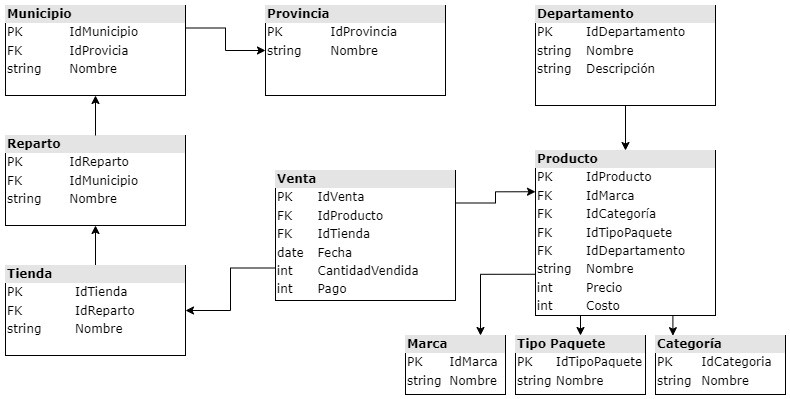
\includegraphics[scale=0.7]{../document/Graphics/retailSales-Transactional.jpg}
    \caption{Sistema Transaccional: Ventas Minoristas}
    \label{fig:retail-transactional}
  \end{figure}

Los archivos que intervienen en este experimento se encuentran en la carpeta \textbf{retail\_sales} del 
directorio \textbf{experiments}. La definición del esquema estrella a poblar se encuentra en el archivo 
\textbf{retailsales.txt}. La figura \ref{fig:retail-Warehouse} muestra la composición de las 
tablas de dimensión y de hechos del esquema estrella propuesto.

\begin{figure}
    \centering
    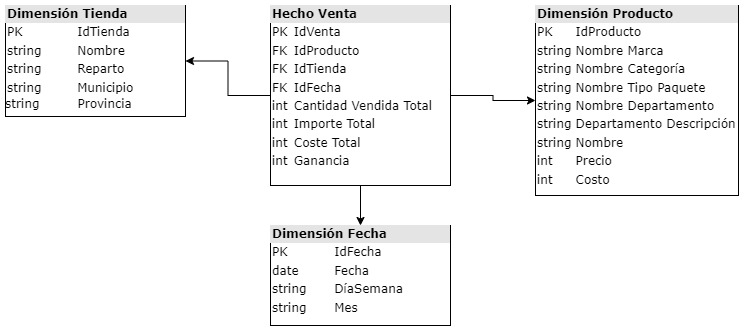
\includegraphics[scale=0.5]{../document/Graphics/retailSales-Data Warehouse.jpg}
    \caption{Almacén de Datos: Ventas Minoristas}
    \label{fig:retail-Warehouse}
\end{figure}

\subsubsection{Fase 1: Exploraci\'on del Crawler y creaci\'on de la base de datos de Neo4j}

Para el esquema de base de datos de la figura \ref{fig:retail-transactional} la base de datos de Neo4j derivada a 
partir de los datos recopilados por el Crawler se muestra en la figura \ref{fig:catalogexp1}.

\begin{figure}
  \centering
  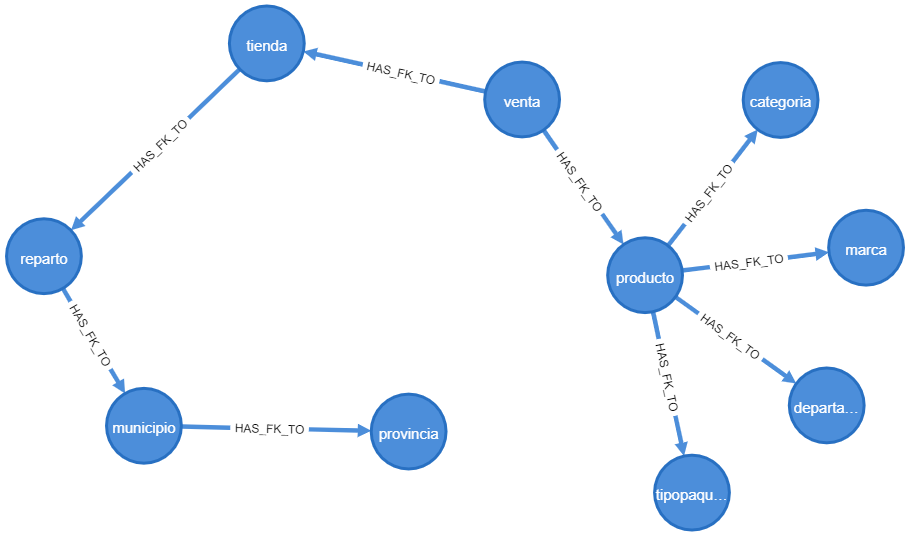
\includegraphics[scale=0.4]{Graphics/graph (1).png}
  \caption{Grafo de Neo4j para el esquema de ventas minoristas}
  \label{fig:catalogexp1}
\end{figure}

\subsubsection{Fase 2: Creaci\'on del grafo de join y \'arboles de join}

A partir del grado de join obtenido en la fase 2 se computan el grafo de join y el \'arbol de 
join que se muestran en la figura \ref{fig:graphjoin1} y en la figura \ref{fig:jointree1}. Para este caso, 
el \'arbol de join es \'unico y coincide  con el grafo de join debido a que el esquema de bases de datos de 
las ventas minoristas no presenta ambiguedades.

\begin{figure}
  \centering
  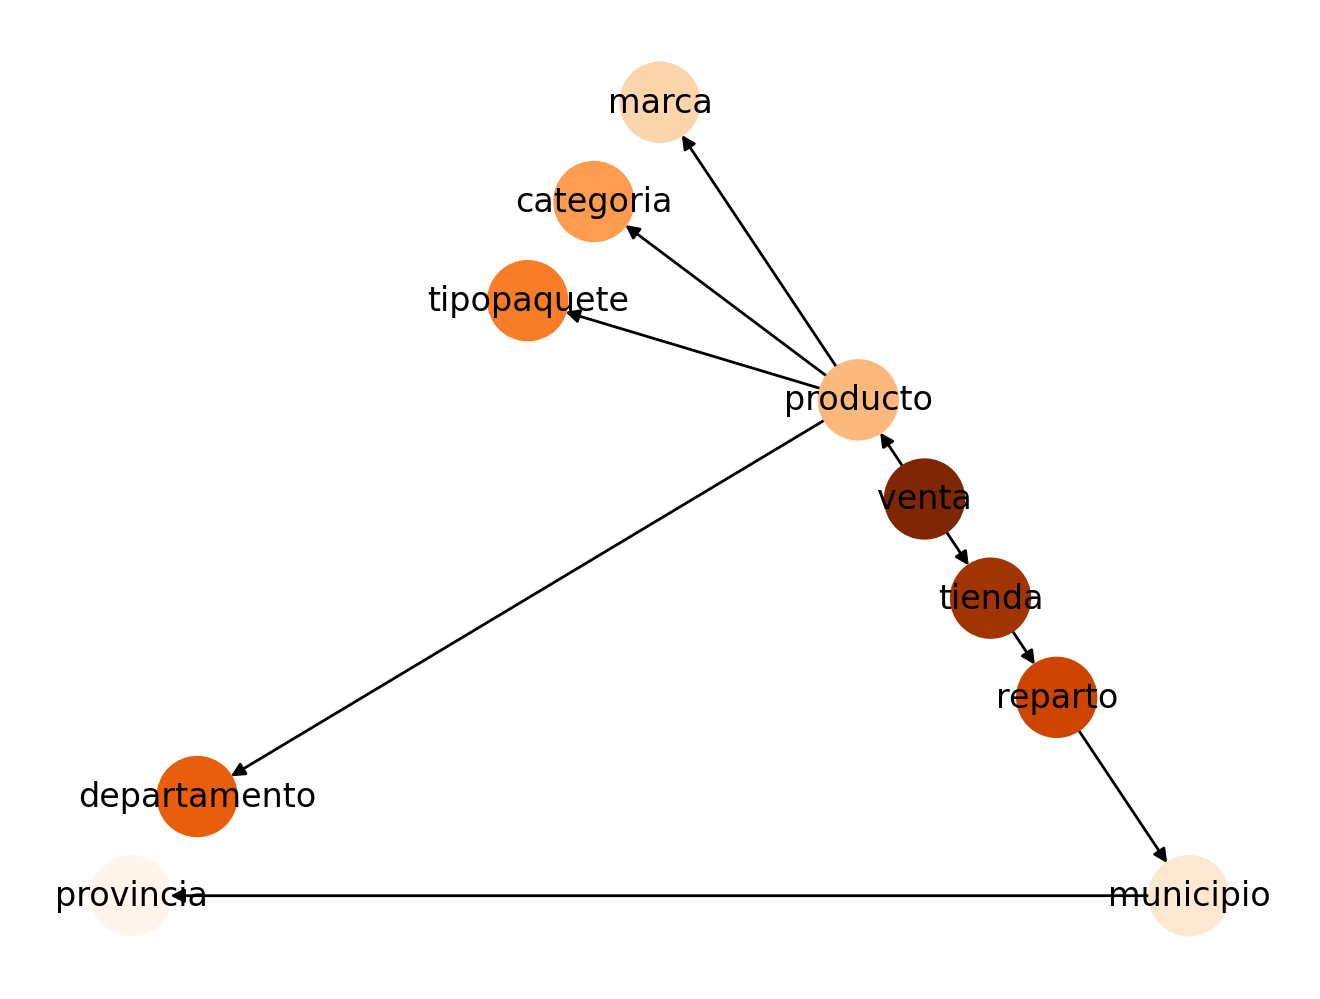
\includegraphics[scale=0.6]{Graphics/joingraph1.png}
  \caption{Grafo de join para el esquema de ventas minoristas}
  \label{fig:graphjoin1}
\end{figure}

\begin{figure}
  \centering
  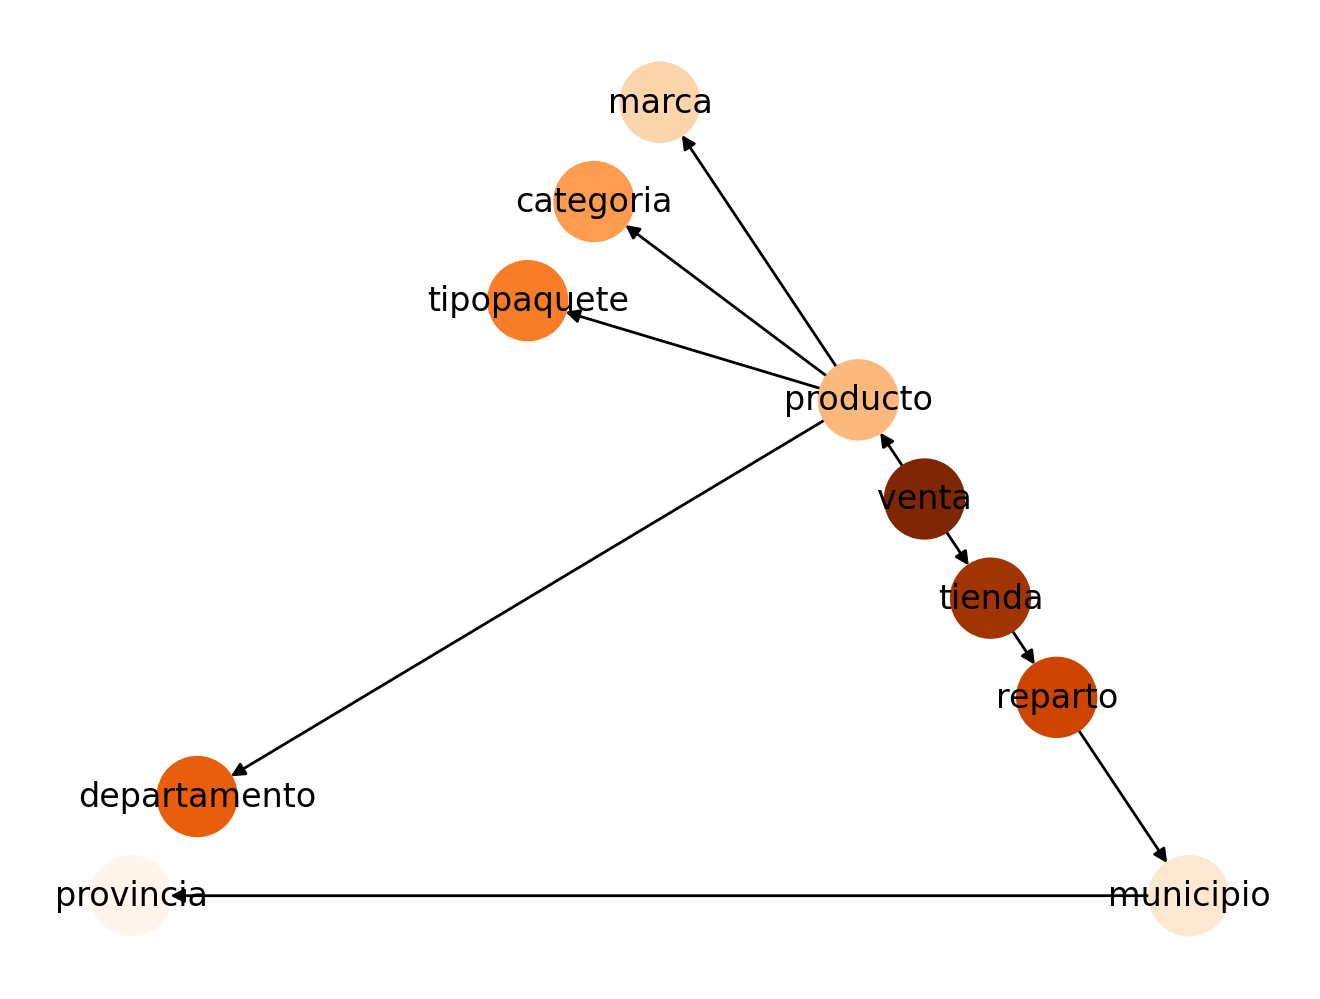
\includegraphics[scale=0.6]{Graphics/jointree1.png}
  \caption{\'Arbol de join para el esquema de ventas minoristas}
  \label{fig:jointree1}
\end{figure}

\subsubsection{Fase 3: Generaci\'on de las consultas}

La selecci\'on de los joins por parte del usuario se efectúa a través de la interfaz de usuario, como se 
muestra en la figura \ref{fig:ui1}. Como solo hay un \'arbol de join hay una \'unica opción de join para 
cada tabla del esquema estrella.

\begin{figure}
  \centering
  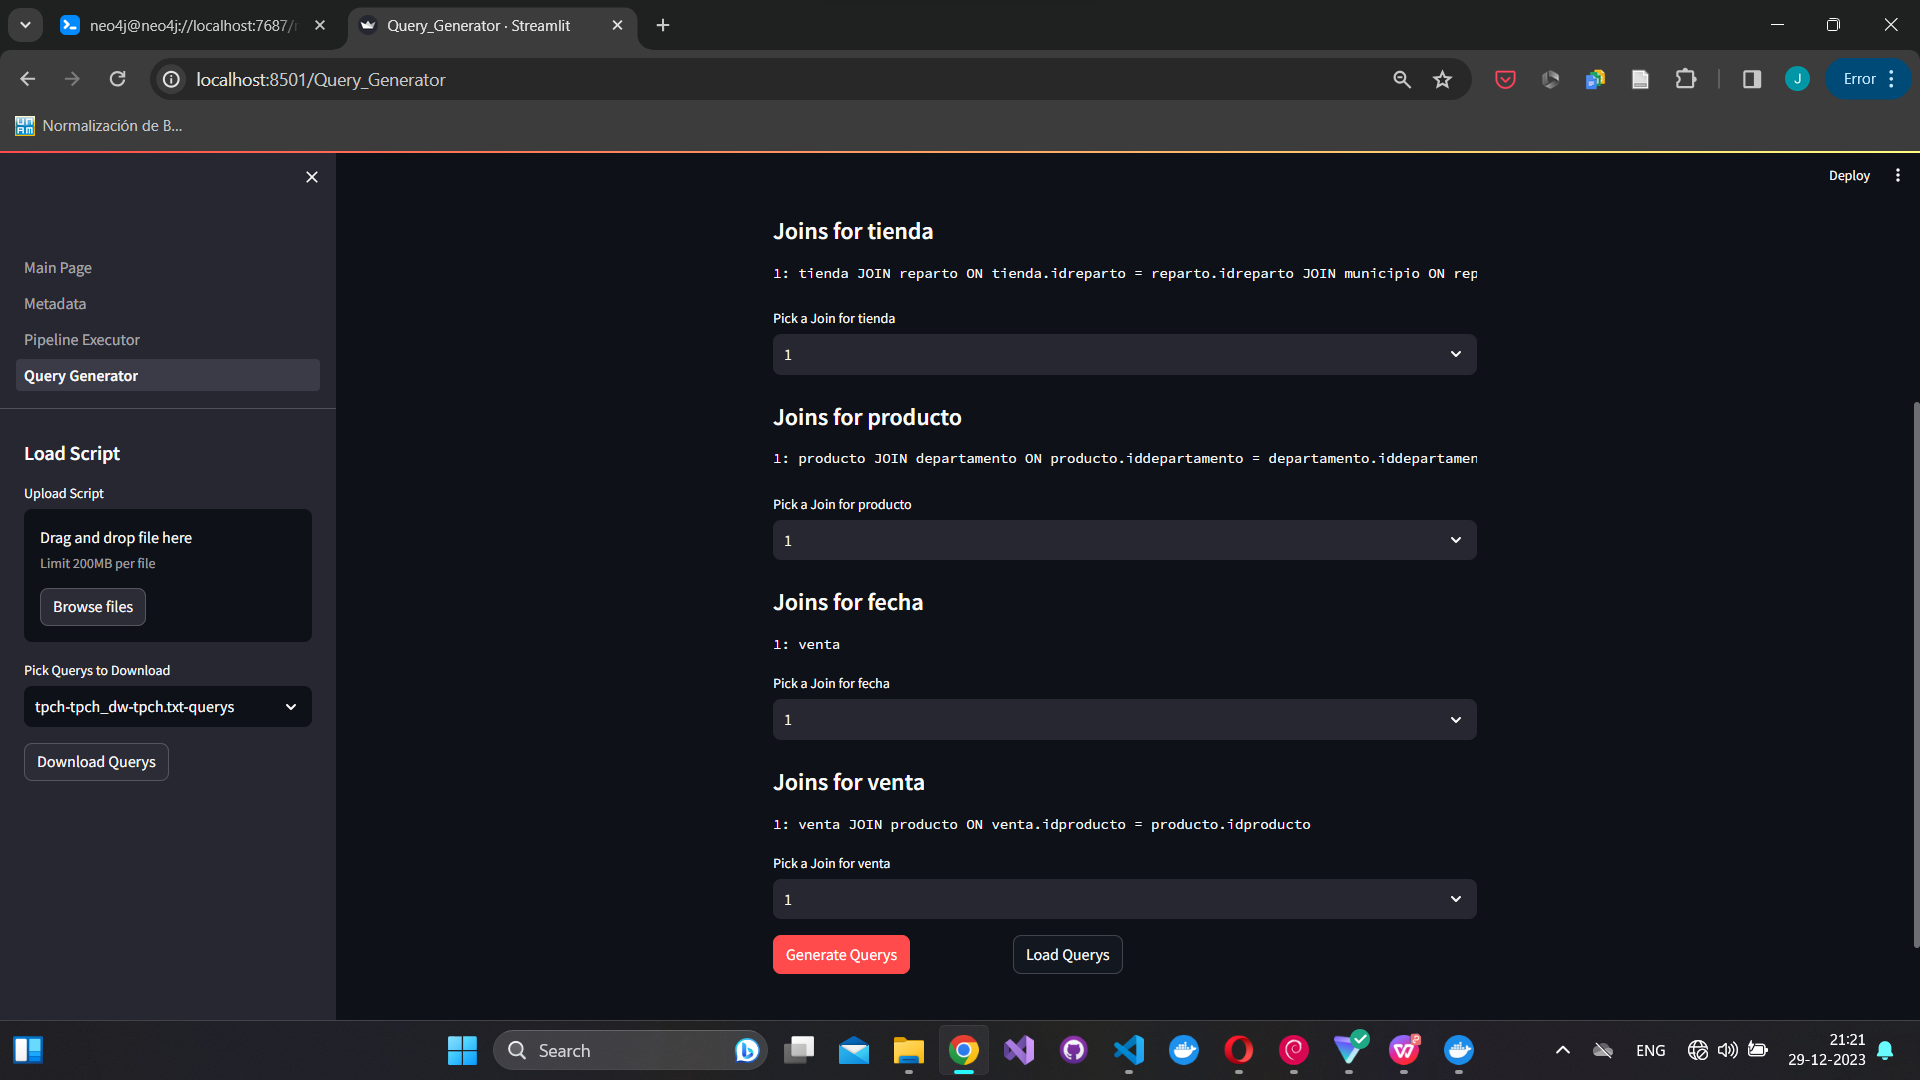
\includegraphics[scale=0.4]{Graphics/ui1.png}
  \caption{Selecci\'on de los joins mediante la interfaz de usuario para la poblaci\'on del almacén de datos derivado de ventas minoristas}
  \label{fig:ui1}
\end{figure}

En la figura \ref{fig:codegen1} se muestra un fragmento de las consultas generadas para la poblaci\'on del esquema 
estrella definido en \textbf{retailsales.txt}.

\begin{figure}
  \centering
  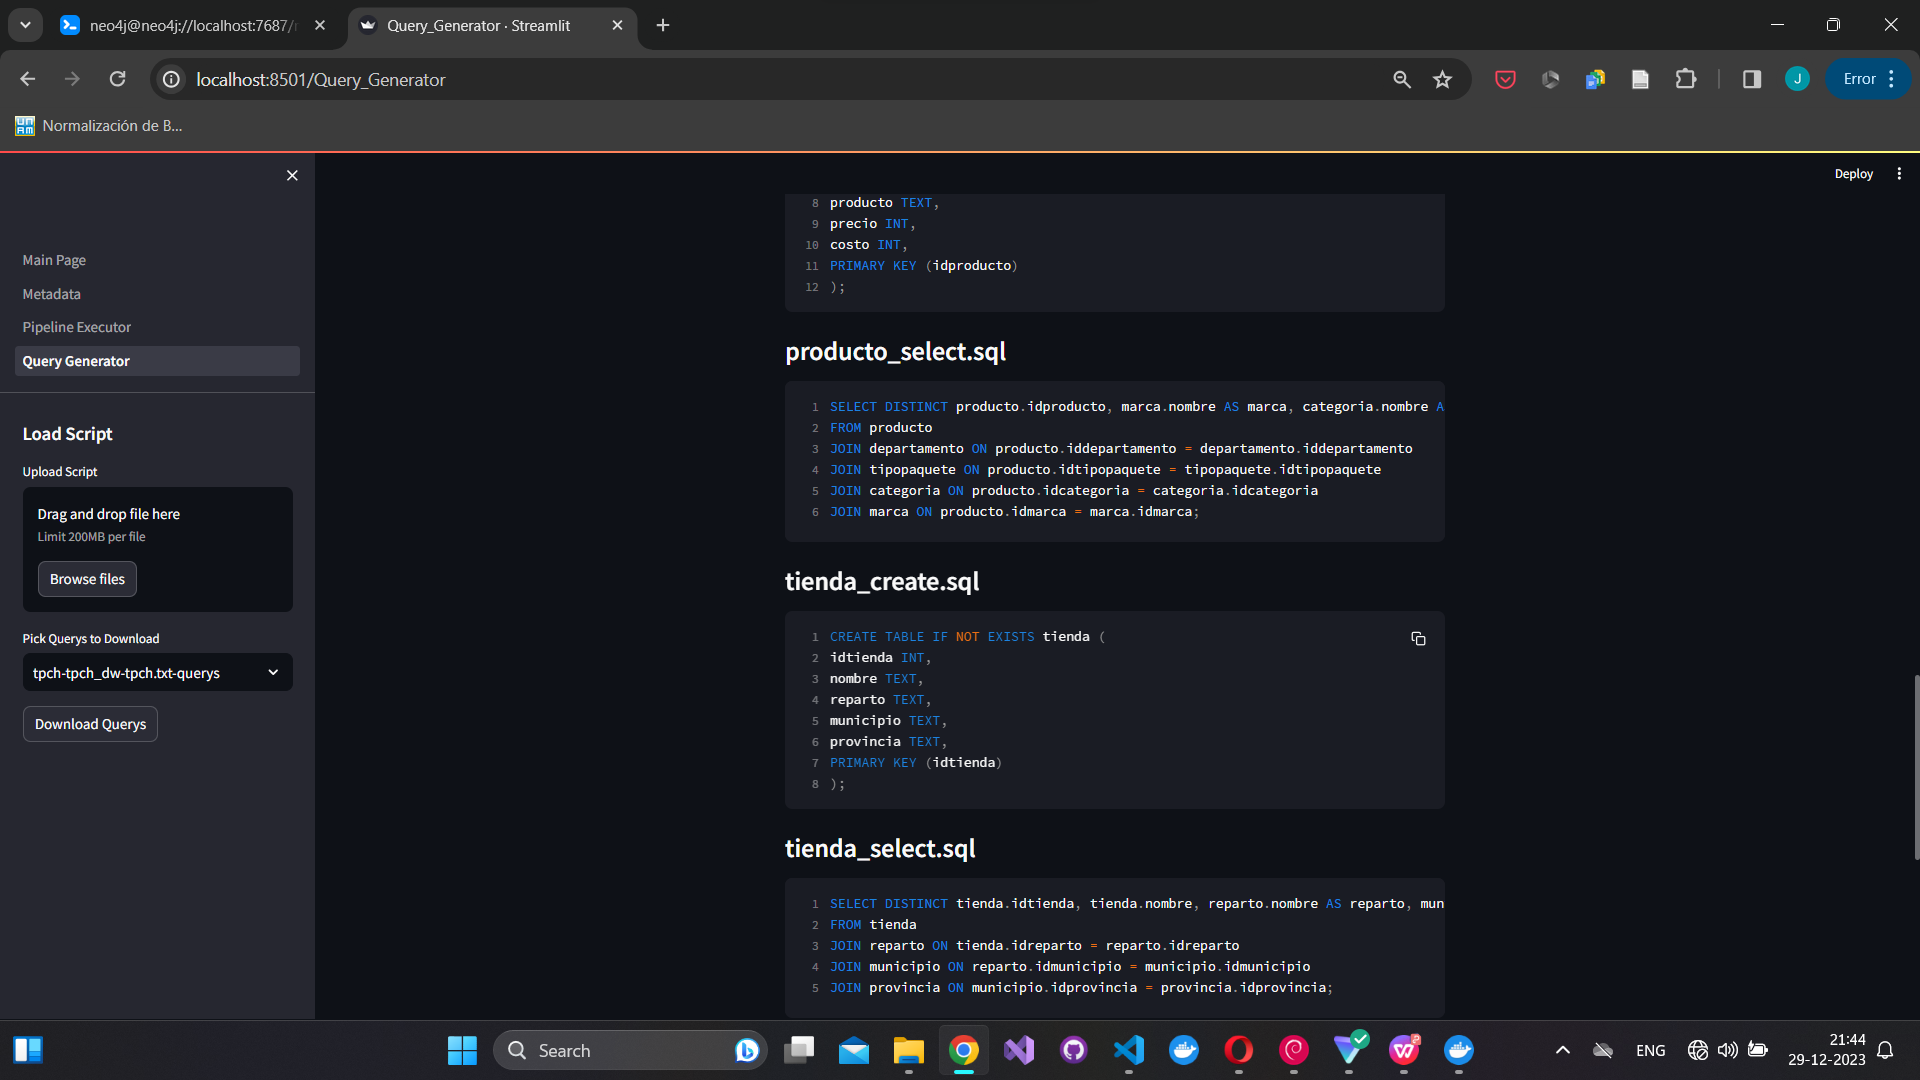
\includegraphics[scale=0.4]{Graphics/generatedquerys1.png}
  \caption{Fragmento de las consultas generadas para la poblaci\'on del almac\'en de datos derivado de ventas minoristas}
  \label{fig:codegen1}
\end{figure}

\subsubsection{Fase 4: Creaci\'on manual del pipeline y poblaci\'on del almac\'en de datos}

El pipeline creado se encuentra en la ruta \textbf{experiments/retail\_sales} con el nombre de 
\textbf{pipeline.py}. La figura \ref{fig:emptypgadmin1} muestra el estado del servidor de bases de 
datos que almacenar\'a la base de datos \textbf{retai\_dw}, nombre del almac\'en de datos definido mediante 
\textbf{retailsales.txt} para la base de datos de ventas minoristas.

\begin{figure}
  \centering
  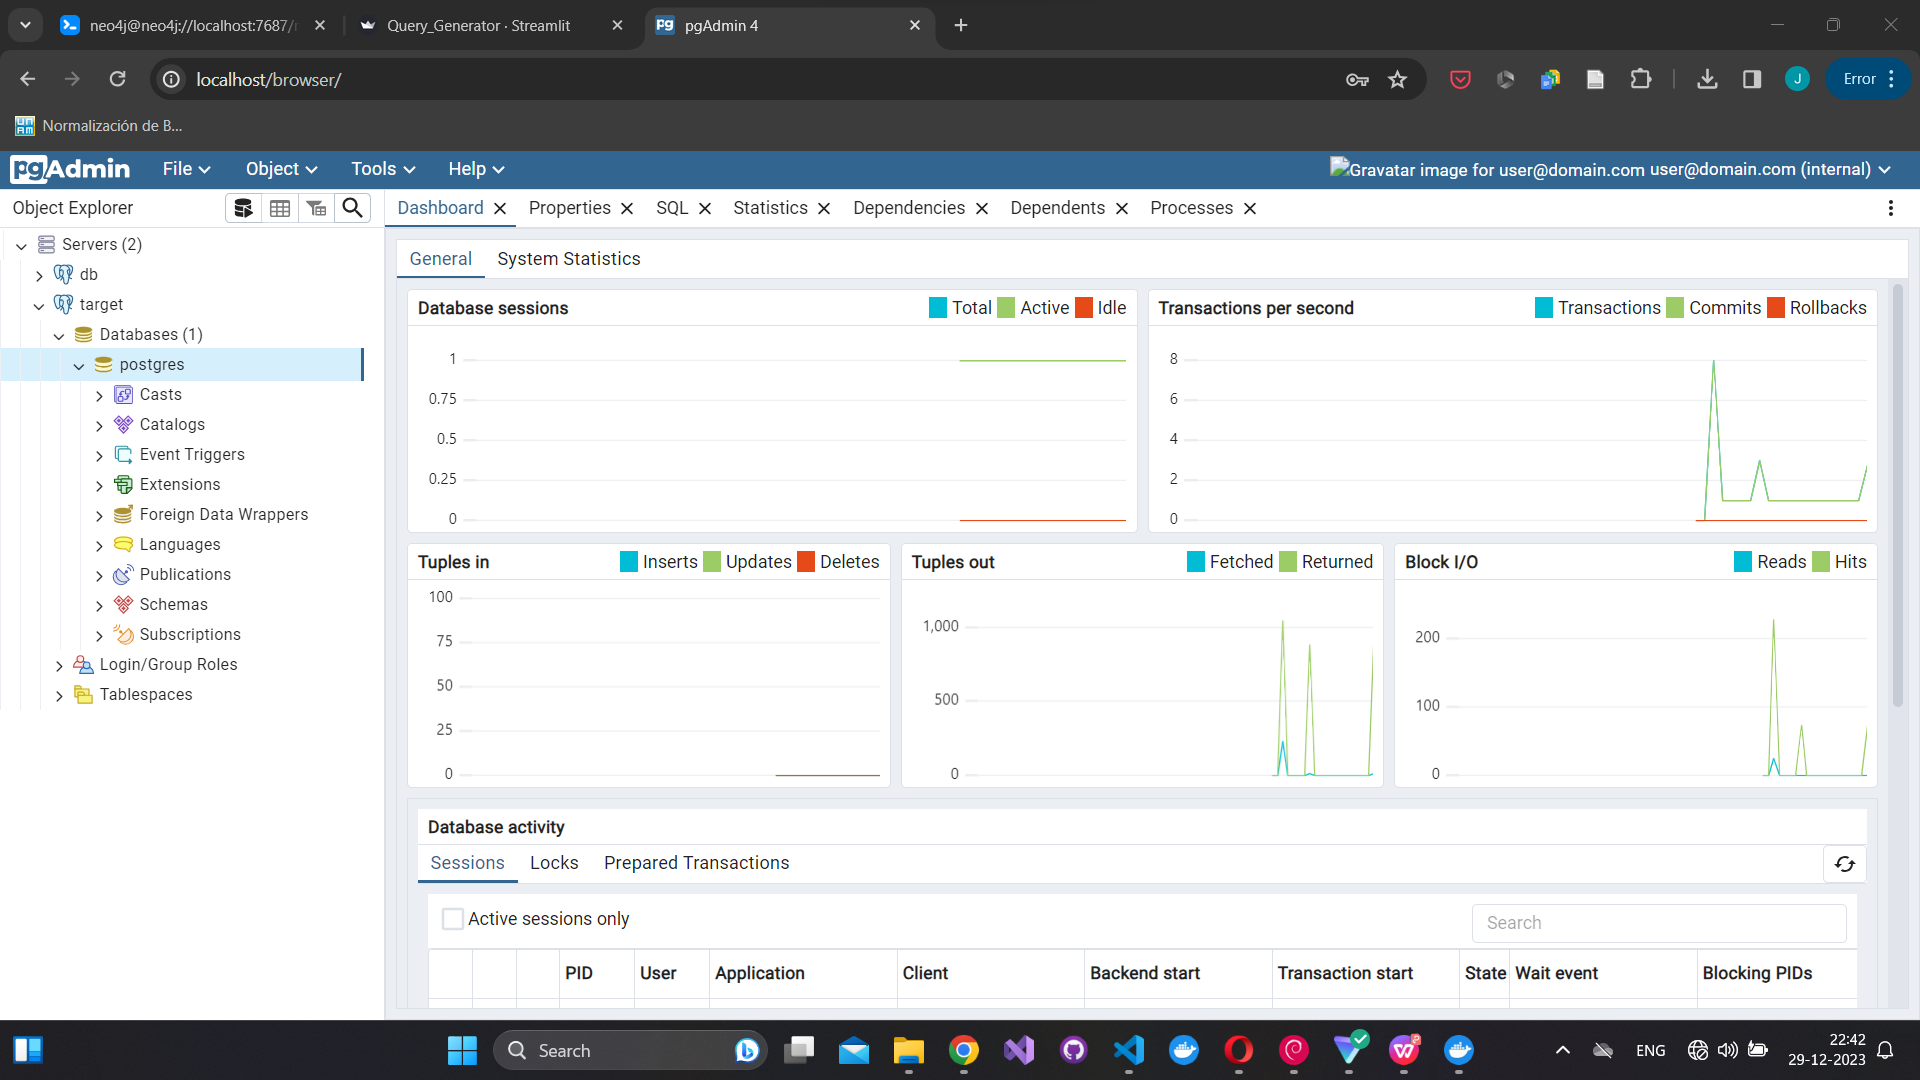
\includegraphics[scale=0.4]{Graphics/emptypgadmin1.png}
  \caption{Estado del servidor de base de datos target antes de la ejecuci\'on del pipeline para ventas minoristas}
  \label{fig:emptypgadmin1}
\end{figure}

La figura  muestra el estado de target luego de la ejecuci\'on del pipeline. La figura muestra como efectivamente 
se han creado y poblado todas la tablas del esquema estrella definido.

